\documentclass[10pt]{article}

\usepackage[USenglish,spanish,es-tabla]{babel}
\usepackage[utf8]{inputenc}
\usepackage{authblk}
\usepackage{csquotes}
\usepackage{lipsum}
\usepackage{amsmath}
\usepackage{amssymb}
\usepackage{gensymb}
\usepackage{textcomp}
\usepackage{enumerate}
\usepackage{enumitem}
\usepackage{bm}
\usepackage{nicefrac}
\usepackage{abstract}
\usepackage{titlesec}
\usepackage{microtype}
\usepackage[margin=2cm]{geometry}
\usepackage{pdfpages}
\usepackage{graphicx}
\usepackage[centerlast]{subfigure}
\usepackage{float}
\usepackage{booktabs}
\usepackage{multicol}
\setlength{\columnsep}{0.75cm}
\spanishdecimal{.}	
\usepackage[justification=centerlast]{caption}
\usepackage{hyperref}
\hypersetup{
    colorlinks=true,
    linkcolor=black,
    filecolor=black,      
    urlcolor=blue,
    citecolor=black,
}
\urlstyle{same}

%\titleformat{\section}
%{\centering\normalfont\bfseries}
%{\thesection.}{0.25cm}{}
%\renewcommand{\thesection}{\Roman{section}}
%
%
%\titleformat{\subsection}
%{\centering\normalfont\scshape}
%{\thesubsection.}{0.25cm}{}
%\renewcommand{\thesubsection}{\thesection.\Roman{subsection}}
%
%\titleformat{\subsubsection}
%{\centering\normalfont\scshape}
%{\thesubsubsection.}{0.25cm}{}
%\renewcommand{\thesubsubsection}{\thesubsection.\Roman{subsubsection}}

%\usepackage[backend=bibtex, bibencoding=ascii,sorting=none]{bibtex}
%\addbibresource{bib.bib}


\usepackage{titling}
\setlength{\droptitle}{-1.5cm}

\setlength\parindent{0pt}

\usepackage{xcolor}

%\pagecolor[rgb]{0,0,0}
%\color[rgb]{1,1,1}

\title{\textbf{Ataque adversarios} \vspace{-0.25em}} 
\author{Enrique David Guzmán Ramírez \vspace{-1em}}
\affil{IIMAS, Universidad Nacional Autónoma de México \vspace{-0.5em}}
\affil{Introducción al Aprendizaje Profundo \vspace{-0.25em} \\  M. en C. Berenice Montalvo Lezama \\ M. en C. Ricardo Montalvo Lezama}

\renewcommand\Affilfont{\normalsize}

\date{{\normalsize \today}}

\begin{document}	

\maketitle

\begin{abstract}
Las redes neuronales profundas son modelos poderosos que se han utilizado ampliamente para lograr un rendimiento cercano al nivel humano en una variedad de tareas. Sin embargo, a pesar de su desempeño superior estudios recientes han encontrado que incluso los modelos del estado del arte son sumamente vulnerables a ataques adversarios. En el presente trabajo se exploran algunos de los algoritmos de ataques adversarios en algunas de las arquitecturas más recientes de visión computacional.
\end{abstract}

\begin{multicols*}{2}

\section{Introducción}

Un ataque adversario es una muestra de datos de entrada que ha sido perturbada
levemente con la intención de hacer fallar a un clasificador

En muchos casos, estas modificaciones pueden ser tan sutiles que un observador humano ni siquiera nota la modificación, pero el clasificador comete un error. Los ejemplos de adversarios plantean problemas de seguridad porque podrían usarse para realizar un ataque a los sistemas de aprendizaje automático, incluso si el atacante no tiene acceso al modelo subyacente.

Con la introducción de modelos de aprendizaje profundo en cada vez más distintos aspectos de nuestra vida, los problemas que estos ataques adversarios pueden ocasionar
son preocupantes.

\begin{figure}[H]
\centering
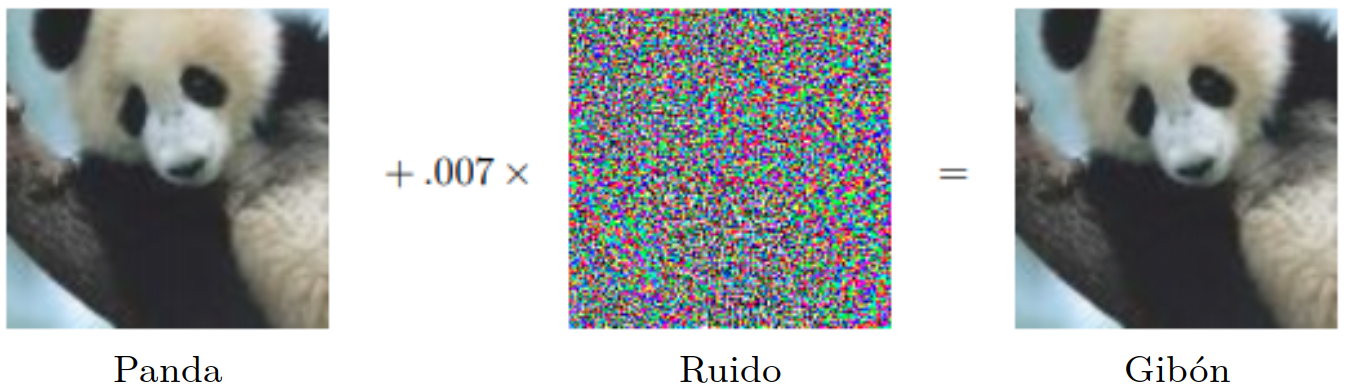
\includegraphics[width=0.99\linewidth]{Images/ejemplo1_anotado.png}
\caption{Ejemplo de ataque adversario. Imagen tomada de \href{https://arxiv.org/pdf/1412.6572.pdf}{\emph{Explaining and harnessing adversarial examples}.}}
\end{figure}

Los escenarios de posibles ataques adversarios se pueden clasificar en diferentes maneras:

\begin{itemize}
\item \textbf{Ataque no dirigido:} el objetivo es hacer que el clasificador prediga una etiqueta incorrecta, la etiqueta incorrecta específica no importa.

\item \textbf{Ataque dirigido:} el objetivo es cambiar la predicción del clasificador a alguna clase objetivo específica.
\end{itemize}

En segundo lugar, los escenarios de ataque se pueden clasificar por la cantidad de conocimiento que el adversario tiene sobre el modelo:

\begin{itemize}
\item \textbf{Caja negra:} el atacante no sabe mucho sobre el modelo, pero puede sondear o consultar el modelo, es decir, darle algunas entradas y observar salidas.

\item \textbf{Caja blanca:} el atacante tiene pleno conocimiento del modelo, como la arquitectura del modelo y los valores de todos los parámetros y pesos entrenables.
\end{itemize}

\subsection{Algoritmos de ataques adversarios}

Hay una multitud de ataques adversarios, pero particularmente usaré los siguientes cuatro:

\begin{enumerate}
\item \textbf{FGSM (Fast Gradient Sign Method)} \cite{FGSM}: la idea es generar el ejemplo adversario $\bm{x}_{\text{adv}}$ de la siguiente forma
%
\[ \bm{x}_{\text{adv}} = \bm{x} + \epsilon \cdot \text{sign}\left( \nabla_{\bm{x}} J(\bm{\theta}, \bm{x}, y) \right). \]
%
donde $\epsilon$ es el orden de la perturbación, $J$ es la función de pérdida (usualmente cross-entropy), $\bm{\theta}$ los pesos del modelo, $\bm{x}$ la imagen original y $y$ la etiqueta.

\item \textbf{PGD (Projected Gradient Descent)} \cite{PGD}: podemos verlo como una variante de varios pasos, donde $\alpha$ es la magnitud de la perturbación en cada paso
%
\[ \bm{x}_{\text{adv}}^{t+1} = \text{Proj}\left( \bm{x}_{\text{adv}}^{t} + \alpha \cdot  \text{sign}\left( \nabla_{\bm{x}} J(\bm{\theta}, \bm{x}, y) \right) \right) \]

\item \textbf{MIFGSM (Momentum Iterative Fast Gradient Sign Method)} \cite{MIFGSM}: algoritmo ganador de esta competencia, inspirados por los optimizadores con momento proponen
%
\[ \bm{x}_{\text{adv}}^{t+1} = \text{Clip}\left( \bm{x}_{\text{adv}}^{t} + \alpha \cdot  \text{sign}(g_{t+1}) \right), \]
%
donde $g_{t+1} = \xi \cdot g_{t} + \dfrac{ \nabla_{\bm{x}} J(\bm{\theta}, \bm{x}, y)}{\left\Vert J(\bm{\theta}, \bm{x}, y) \right\Vert} $, donde $\xi$ es un factor de decaimiento.

\item \textbf{One Pixel Attack} \cite{OnePixel}: plantea el problema como un problema de optimización
%
\begin{align*}
	& \hspace{2em} \max_{\bm{x}_{\text{adv}}} f_{\text{adv}} (\bm{x} + \bm{x}_{\text{adv}}), \\
	& \text{con la restricción } \left\Vert \bm{x}_{\text{adv}} \right\Vert \leq d,
\end{align*}
%
donde $d = 1$ para el caso de un ataque a un pixel. Particularmente proponen resolver este problema de optimización con \emph{evolución diferencial}.

\end{enumerate}

\section{Objetivo}

El objetivo del proyecto es explorar y desarrollar algunas de las técnicas usadas para generar ataques adversarios así como explorar algunos de los métodos de defensa que existen.

\section{Propuesta de solución}

Hay una variedad de arquitecturas preentrenadas en PyTorch con el conjunto de datos de ImageNet que sirven a la perfección para esta tarea, particularmente usaré las siguientes

\begin{itemize}
	\item AlexNet
	\item Resnet18
	\item Inception v3
	\item MobileNet v2
\end{itemize}

Con estas arquitecturas y métodos se exploraron los ataques y defensas adversarias.

\begin{itemize}
\item Para los ataques de caja blanca los ejemplos adversarios se hacen a la medida para cada modelo, posteriormente podemos evaluar el accuracy con cada ataque.

\item Para el ataque de caja negra se generaron los ejemplos adversarios con Inception v3 y se le pasaron a MobileNet v2.

\item Para las defensas usé una versión modificada de MobileNet v2 para que use CIFAR10. Entrené desde cero usando el dataset de entrenamiento de CIFAR10 y posteriomente entrené otro modelo agregando 20,000 ejemplos adversarios al dataset, lo que hace que el modelo sea más robusto a ataques adversarios. 
\end{itemize}

\section{Resultados}

Con los ataques de caja blanca, donde los ejemplos adversarios se hacen a la medida de cada modelo, la disminución en el accuracy es enorme.

\begin{table}[H]
	\centering
	\resizebox{\linewidth}{!}{%
		\begin{tabular}{@{}cccccc@{}}
			\toprule
			\textbf{Modelo} & \textbf{\begin{tabular}[c]{@{}c@{}}Limpio \\ (acc@1/acc@5)\end{tabular}} & \textbf{\begin{tabular}[c]{@{}c@{}}FGSM \\ (acc@1/acc@5)\end{tabular}} & \textbf{\begin{tabular}[c]{@{}c@{}}PGD \\ (acc@1/acc@5)\end{tabular}} & \textbf{\begin{tabular}[c]{@{}c@{}}MIFGSM \\ (acc@1/acc@5)\end{tabular}} & \textbf{\begin{tabular}[c]{@{}c@{}}OnePixel \\ (acc@1/acc@5)\end{tabular}} \\ \midrule
			AlexNet         & 60.9 / 84.6                                                              & 6.0 / 28.6                                                             & 2.9 / 19.3                                                            & 3.5 / 21.0                                                               & 58.3 / 83.4                                                                \\
			ResNet-18       & 82.5 / 95.4                                                              & 3.5 / 24.3                                                             & 0.8 / 14.6                                                            & 1.0 / 13.5                                                               & 78.7 / 94.5                                                                \\
			Inception v3    & 76.5 / 93.1                                                              & 10.8 / 39.3                                                            & 3.9 / 28.1                                                            & 5.1 / 27.6                                                               & 70.1 / 91.8                                                                \\
			MobileNet v2    & 85.0 / 97.3                                                              & 3.5 / 24.4                                                             & 0.5 / 11.3                                                            & 0.6 / 8.8                                                                & 81.4 / 96.6                                                                \\ \bottomrule
		\end{tabular}%
	}
	\caption{Ataques de caja blanca.}
\end{table}

\begin{figure}[H]
	\centering
	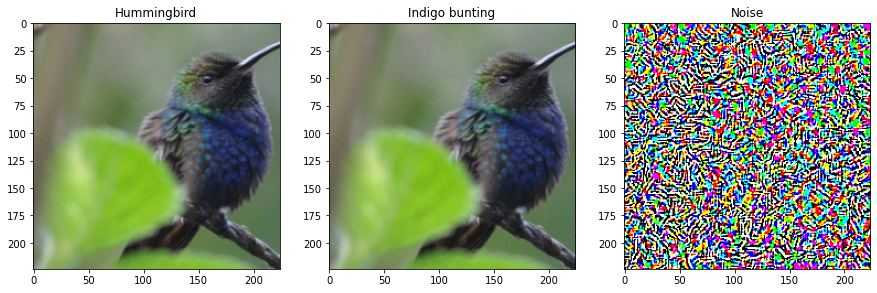
\includegraphics[width=0.99\linewidth]{Images/hummingbird_alexnet_FGSM.png}
	\caption{Ataque de caja blanca a AlexNet con FGSM.}
\end{figure}

\begin{figure}[H]
	\centering
	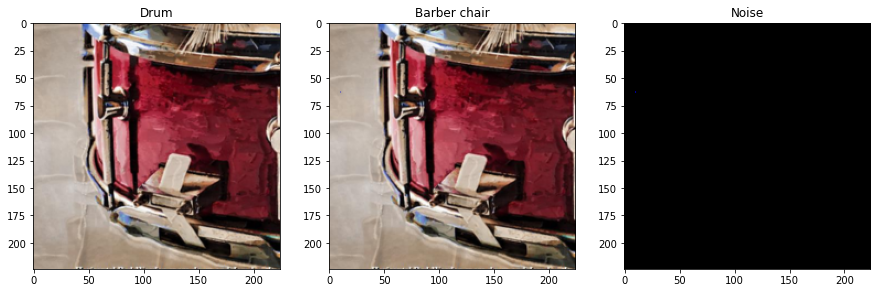
\includegraphics[width=0.99\linewidth]{Images/inception_v3_OnePixel.png}
	\caption{Ataque de caja blanca a Inception v3 con OnePixel.}
\end{figure}

En el caso del ataque de caja negra hice los ataques más agresivos, aunque no es tan efectivo como un ataque de caja blanca, se logra bajar considerablemente el accuracy del modelo.

\begin{table}[H]
	\centering
	\resizebox{\linewidth}{!}{%
		\begin{tabular}{@{}cccccc@{}}
			\toprule
			\textbf{Modelo} & \textbf{\begin{tabular}[c]{@{}c@{}}Limpio \\ (acc@1/acc@5)\end{tabular}} & \textbf{\begin{tabular}[c]{@{}c@{}}FGSM \\ (acc@1/acc@5)\end{tabular}} & \textbf{\begin{tabular}[c]{@{}c@{}}PGD \\ (acc@1/acc@5)\end{tabular}} & \textbf{\begin{tabular}[c]{@{}c@{}}MIFGSM \\ (acc@1/acc@5)\end{tabular}} & \textbf{\begin{tabular}[c]{@{}c@{}}OnePixel \\ (acc@1/acc@5)\end{tabular}} \\ \midrule
			MobileNet v2    & 85.0 / 97.3                                                              & 51.7 / 78.3                                                            & 59.4 / 82.9                                                           & 56.3 / 81.5                                                              & 83.5 / 97.0                                                                \\ \bottomrule
		\end{tabular}%
	}
	\caption{Ataque de caja negra a MobileNet v2.}
\end{table}

\begin{figure}[H]
	\centering
	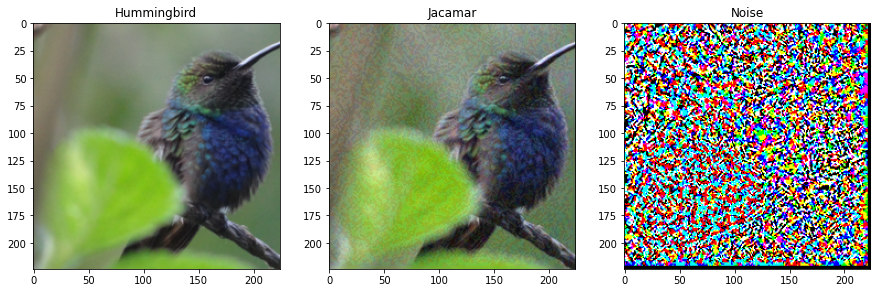
\includegraphics[width=0.99\linewidth]{Images/hummingbird_blackbox_FGSM.png}
	\caption{Ataque de caja negra a MobileNet v2 con FGSM.}
\end{figure}

\begin{figure}[H]
	\centering
	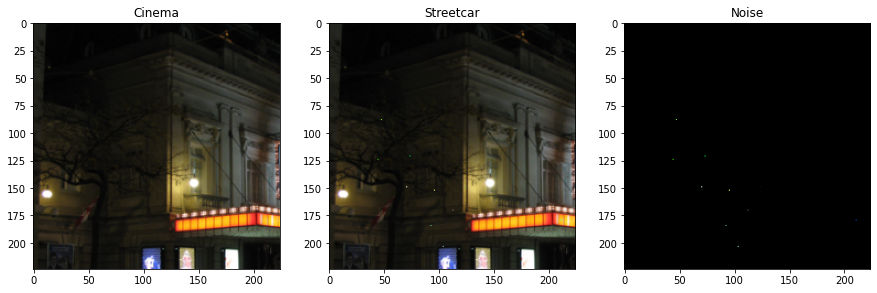
\includegraphics[width=0.99\linewidth]{Images/blackbox_OnePixel.png}
	\caption{Ataque de caja negra a MobileNet v2 con OnePixel.}
\end{figure}

En cuanto al entrenamiento con ejemplos adversarios, se confirma que es una técnica sencilla pero eficiente.

\begin{table}[H]
	\centering
	\resizebox{\linewidth}{!}{%
		\begin{tabular}{@{}cccccc@{}}
			\toprule
			\textbf{Modelo}          & \textbf{\begin{tabular}[c]{@{}c@{}}Limpio \\ (accuracy)\end{tabular}} & \textbf{\begin{tabular}[c]{@{}c@{}}FGSM \\ (accuracy)\end{tabular}} & \textbf{\begin{tabular}[c]{@{}c@{}}PGD \\ (accuracy)\end{tabular}} & \textbf{\begin{tabular}[c]{@{}c@{}}MIFGSM \\ (accuracy)\end{tabular}} & \textbf{\begin{tabular}[c]{@{}c@{}}OnePixel \\ (accuracy)\end{tabular}} \\ \midrule
			MobileNet v2             & 81.68                                                                 & 37.03                                                               & 28.29                                                              & 31.27                                                                 & 63.17                                                                   \\
			MobileNet v2 adversarial & 80.62                                                                 & 77.44                                                               & 77.49                                                              & 77.35                                                                 & 77.58                                                                   \\ \bottomrule
		\end{tabular}%
	}
	\caption{Entrenamiento sin y con ejemplos adversarios en CIFAR10 con una versión modificada de MobileNet v2.}
\end{table}

\begin{figure}[H]
	\centering
	\subfigure[Ataque adversario con FGSM a MobileNet v2 entrenada sin ejemplos adversarios.]{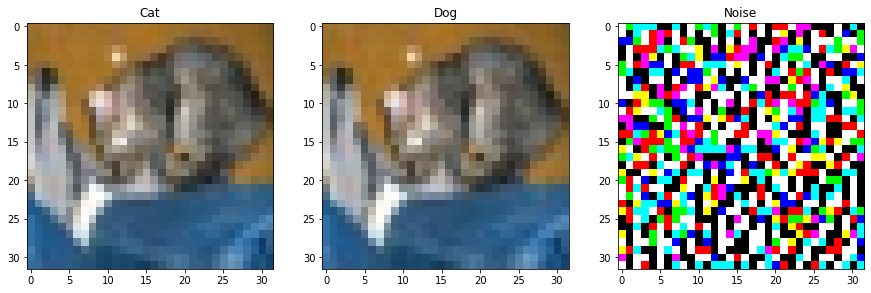
\includegraphics[width=0.99\linewidth]{Images/cifar10_FGSM.png}}
	\subfigure[Ataque adversario con FGSM a MobileNet v2 entrenada con ejemplos adversarios.]{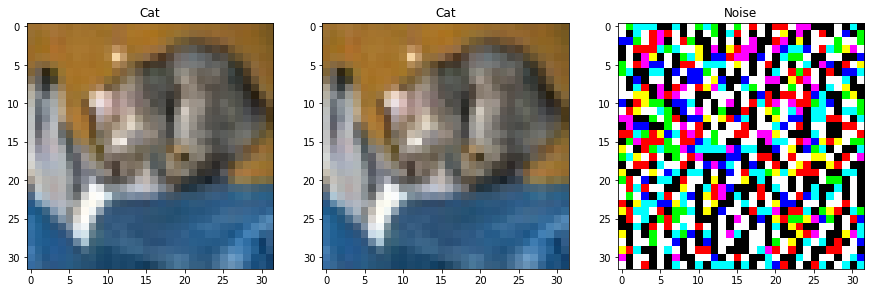
\includegraphics[width=0.99\linewidth]{Images/cifar10_adversarial_FGSM.png}}
	\caption{Entrenamiento adversario.}
\end{figure}

\section{Conclusiones}

\begin{itemize}
	\item Los ataques adversarios son un fenómeno interesante y un problema importante en la seguridad del aprendizaje automático, por lo que es relevante hacer notar a la comunidad de este problema.
	
	\item Ataques relativamente simples pueden engañar fácilmente incluso a los modelos más recientes sin que un humano llegue a notarlos.
	
	\item El estudio de estos ataques a su vez nos puede ayudar a generar defensas para hacer a los modelos más robustos, confiables y seguros.
\end{itemize}

\bibliographystyle{ieeetr}
\bibliography{bib.bib}

\end{multicols*}

\end{document}
